\documentclass[12pt,oneside]{article} % Uma Coluna e lingua portuguesa
%\usepackage[T1]{fontenc}        % Permite digitar os acentos de forma normal
\usepackage[utf8]{inputenc}
%\usepackage[english]{babel}
% \usepackage[portuges,brazil]{babel}
\usepackage[brazilian]{babel}

%\usepackage[latin1]{inputenc}
\usepackage[dvips]{graphicx}    % Permite Gráficos
%\usepackage{times}    % Fonte Times
\usepackage{fancyhdr}
\usepackage{array}
\usepackage{multicol}
\usepackage[colorlinks=true,linkcolor=blue,urlcolor=blue]{hyperref}
\usepackage{nomencl}    % glossario
\usepackage{amssymb}
\usepackage{amsmath}
\usepackage[compact]{titlesec}
\usepackage{wrapfig}
\usepackage{color}
\usepackage{listingsutf8}

% Configuração do estilo de código c++ do listingsutf8
\definecolor{clr-background}{RGB}{255,255,255}
\definecolor{clr-text}{RGB}{0,0,0}
\definecolor{clr-string}{RGB}{163,21,21}
\definecolor{clr-namespace}{RGB}{0,0,0}
\definecolor{clr-preprocessor}{RGB}{128,128,128}
\definecolor{clr-keyword}{RGB}{0,0,255}
\definecolor{clr-type}{RGB}{43,145,175}
\definecolor{clr-variable}{RGB}{0,0,0}
\definecolor{clr-constant}{RGB}{111,0,138} % macro color
\definecolor{clr-comment}{RGB}{0,128,0}
\definecolor{clr-linenumber}{RGB}{128,128,128}

\lstdefinestyle{cppStyle}{
    language=C++,
    backgroundcolor=\color{clr-background},
    basicstyle=\ttfamily\footnotesize\color{clr-text}, % any text
    stringstyle=\color{clr-string},
    identifierstyle=\color{clr-variable}, % just about anything that isn't a directive, comment, string or known type
    commentstyle=\color{clr-comment},
    directivestyle=\color{clr-preprocessor}, % preprocessor commands
    % listings doesn't differentiate between types and keywords (e.g. int vs return)
    keywordstyle=\color{clr-type},
    keywordstyle={[2]\color{clr-constant}}, % you'll need to define these or use a custom language
    numberstyle=\tiny\color{clr-linenumber},
    %numbers=left,
    showspaces=false,
    showtabs=false,
    showstringspaces=false,
    breaklines=true,
    tabsize=2,
    texcl=true
}

%=======================================================================

% Hifenização das palavras desconhecidas pelo LaTeX
%\hyphenation{}
\paperheight    297mm
\paperwidth     210mm
\voffset         -15mm
\headheight      15pt %% tamanho de letra
\headsep         5mm  %% para o início do texto
\oddsidemargin  -3.0mm
\evensidemargin -3.0mm
\textwidth      167.0mm
\topmargin      005.0mm
\textheight     240.0mm
\footskip       10.0mm

\title{PPCI 2024 - Maratona de Programação}

\author{Maratona de Programação}
\date{19 de outubro de 2024}
\usepackage{indentfirst}
\usepackage{subfig}

\parindent=0pt
\setlength{\parskip}{7pt plus 1pt minus 2pt}
\titlespacing{\section}{0pt}{*0}{*0}
\titlespacing{\subsection}{0pt}{*0}{*0}
\titlespacing{\subsubsection}{0pt}{*0}{*0}

\begin{document}

\begin{center}
\textbf{\Huge PPCI 2024 - Maratona de Programação} \\
\vspace{0.2cm}
\textit{19 de outubro de 2024} \\
\vspace{1.0cm}
%\textbf{Sevidor BOCA:} \\
%\texttt{\large http://maratona.c3sl.ufpr.br/boca/} \\
%\vspace{1.0cm}
\begin{figure}[h!]
	\centering
 
\includegraphics[scale=0.95]{capa.png}
\end{figure}
\vspace{1.0cm}
%\textbf{Organizadores:}\\
%{\small Flávio Zavan} \\
%{\small Ricardo Oliveira} \\
\vspace{1.0cm}
\end{center}

\clearpage

\pagestyle{fancy}
\renewcommand{\footrulewidth}{0.7pt}
\renewcommand{\headrulewidth}{0.7pt}
\lhead{PPCI 2024}
\chead{Maratonas de Programação}
\rhead{19 de outubro de 2024}
\cfoot{\thepage}

\newpage
\section*{A: Arremesso de Triângulo} %tle=1
O algoritmo de Manacher[1] encontra, para cada posição $i$ da string, o maior
valor de $j$ tal que $s[i-j..i+j]$ é palíndrome, e o maior valor de $j'$ tal que
$s[i-j'+1..i+j']$ é palíndrome (isto é, o algoritmo consegue determinar, para cada
posição da string, o tamanho da substring palíndrome maximal cujo centro ocorre
naquela posição, tanto a de tamanho ímpar ($j$) quanto a de tamanho par ($j'$)). O algoritmo tem complexidade $O(N)$.

A figura abaixo exemplifica a solução para o exemplo dado no enunciado. O
tamanho obtido pelo algoritmo de Manacher é representado em vermelho:

\begin{center}
    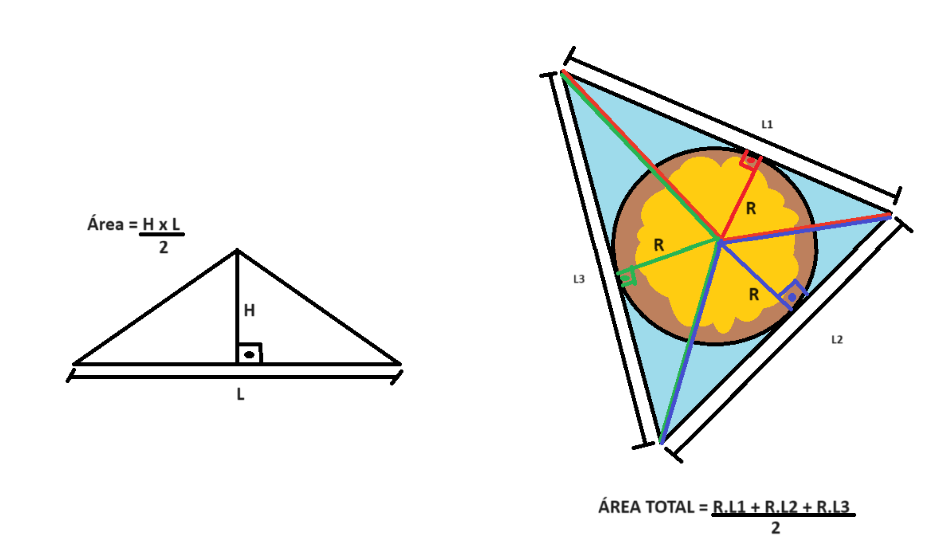
\includegraphics[scale=0.65]{drawkcab/editorial.png}
\end{center}

O próximo passo é determinar o maior valor total possível para cada substring
palindrome maximal. Note que, para substrings de tamanho par, isto é dado por
duas vezes a soma do prefixo de maior soma na segunda metade da substring, e
que, para substrings de tamanho ímpar, é dado por essa soma mais o valor da
letra em seu centro. Na figura exemplificada acima, a resposta é dada por duas vezes a soma do prefixo de maior
soma em $[-10,15,11,-20]$ (que é 16, dado pela soma de $[-10,15,11]$).

Esta soma
pode ser obtida em $O(\lg N)$ através da construção de uma Árvore de
Segmentos adaptada para responder essas consultas, conforme descrito em [2].

Complexidade total: $O(N\lg N)$.

[1] \url{https://cp-algorithms.com/string/manacher.html}

[2] \url{https://www.geeksforgeeks.org/maximum-prefix-sum-given-range/}

%\lstinputlisting[title=\large\textbf{arremesso.cpp}, style=cppStyle]{arremesso/arremesso.cpp}

\newpage
\section*{B: Bloons} %tle=1
Para resolver o problema, pode-se utilizar programação dinâmica, considerando cada balão de forma independente. Assim, para cada balão, queremos encontrar a quantidade mínima de dardos para destruí-lo, usando os dados disponíveis. Vamos definir:

\[
\begin{align*}
dp[x]: &\ \text{o número mínimo de dardos necessários para destruir um balão com} \\
       &\ \text{resistência } x.
\end{align*}
\]

\[
dp[0] = 0,
\]
já que para um balão com 0 camadas de resistência, não precisamos de nenhum dardo.

Para valores maiores de resistência, definimos \(dp[x] = \infty\), representando que ainda não sabemos como destruir aquele balão.

O estado de transição será:
Para cada camada \(x\) e cada macaco distinto com dano \(d_j\), se for possível usar o macaco \((x \geq d_j)\), então podemos atualizar o número mínimo de dardos:

\[
dp[x] = \min(dp[x], dp[x - d_j] + 1)
\]

Essa transição verifica se podemos destruir o balão com resistência \(x\) usando um dardo que destrói \(d_j\) camadas e o número mínimo de dardos necessários para destruir um balão de resistência \(x - d_j\).

Assim, para cada dardo \(d_j\) disponível, atualizamos o array \(dp\) para cada resistência de balão possível \(dp[x]\). Se, ao final do processo, \(dp[h_i] = \infty\), isso significa que não é possível destruir o balão de resistência \(h_i\) com os dardos disponíveis, então retornamos -1. Caso contrário, somamos o total de dardos mínimos necessários para destruir todos os balões.


\newpage

\section*{Código}

\begin{lstlisting}[language=C++]
#include <bits/stdc++.h>
#define ll long long
using namespace std;
const ll INF = INT_MAX;

int main() {
    ll N, K;
    ll MaximoDeCamadas = 1000;
    
    cin >> N >> K;
    
    vector<ll> baloes(N);
    vector<ll> macacos(K);

    for (ll i = 0; i < N; ++i) {
        cin >> baloes[i];
    }

    for (ll i = 0; i < K; ++i) {
        cin >> macacos[i];
    }
    
    vector<ll> dp(MaximoDeCamadas + 1, INF);
    dp[0] = 0;

    for (ll h = 1; h <= MaximoDeCamadas; ++h) {
        for (ll d : macacos) {
            if (h >= d && dp[h - d] != INF) {
                dp[h] = min(dp[h], dp[h - d] + 1);
            }
        }
    }

    ll total_macacos = 0;
    for (ll h : baloes) {
        if (dp[h] == INF) {
            cout << -1 << endl;
            return 0;
        }
        total_macacos += dp[h];
    }
    
    cout << total_macacos << endl;
    return 0;
}
\end{lstlisting}

Complexidade O(N+K)

%\lstinputlisting[title=\large\textbf{bloons.cpp}, style=cppStyle]{bloons/bloons.cpp}

%\newpage
%\section*{C: Cofre Break} %tle=1
%O algoritmo de Manacher[1] encontra, para cada posição $i$ da string, o maior
valor de $j$ tal que $s[i-j..i+j]$ é palíndrome, e o maior valor de $j'$ tal que
$s[i-j'+1..i+j']$ é palíndrome (isto é, o algoritmo consegue determinar, para cada
posição da string, o tamanho da substring palíndrome maximal cujo centro ocorre
naquela posição, tanto a de tamanho ímpar ($j$) quanto a de tamanho par ($j'$)). O algoritmo tem complexidade $O(N)$.

A figura abaixo exemplifica a solução para o exemplo dado no enunciado. O
tamanho obtido pelo algoritmo de Manacher é representado em vermelho:

\begin{center}
    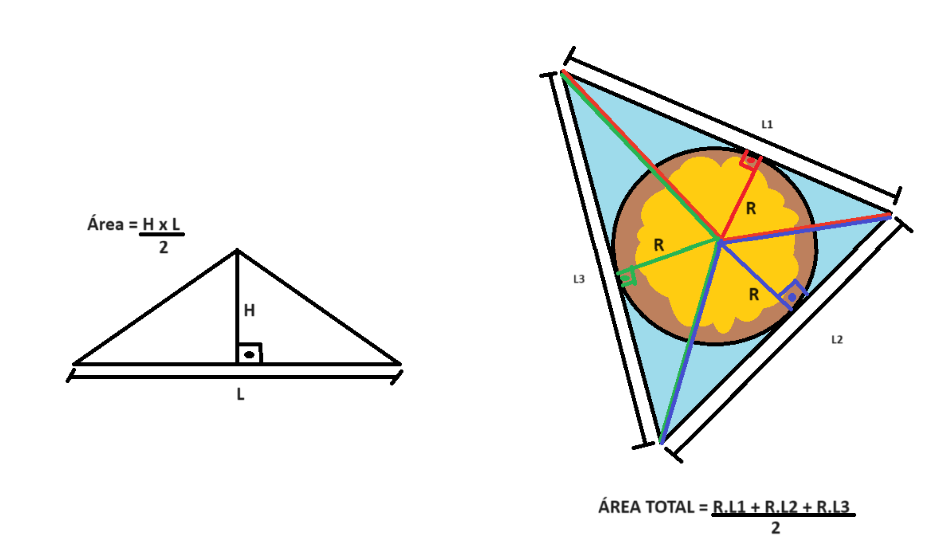
\includegraphics[scale=0.65]{drawkcab/editorial.png}
\end{center}

O próximo passo é determinar o maior valor total possível para cada substring
palindrome maximal. Note que, para substrings de tamanho par, isto é dado por
duas vezes a soma do prefixo de maior soma na segunda metade da substring, e
que, para substrings de tamanho ímpar, é dado por essa soma mais o valor da
letra em seu centro. Na figura exemplificada acima, a resposta é dada por duas vezes a soma do prefixo de maior
soma em $[-10,15,11,-20]$ (que é 16, dado pela soma de $[-10,15,11]$).

Esta soma
pode ser obtida em $O(\lg N)$ através da construção de uma Árvore de
Segmentos adaptada para responder essas consultas, conforme descrito em [2].

Complexidade total: $O(N\lg N)$.

[1] \url{https://cp-algorithms.com/string/manacher.html}

[2] \url{https://www.geeksforgeeks.org/maximum-prefix-sum-given-range/}

%\lstinputlisting[title=\large\textbf{cofre-break.cpp}, style=cppStyle]{cofre-break/cofre-break.cpp}

\newpage
\section*{D: Double Casting} %tle=1
O algoritmo de Manacher[1] encontra, para cada posição $i$ da string, o maior
valor de $j$ tal que $s[i-j..i+j]$ é palíndrome, e o maior valor de $j'$ tal que
$s[i-j'+1..i+j']$ é palíndrome (isto é, o algoritmo consegue determinar, para cada
posição da string, o tamanho da substring palíndrome maximal cujo centro ocorre
naquela posição, tanto a de tamanho ímpar ($j$) quanto a de tamanho par ($j'$)). O algoritmo tem complexidade $O(N)$.

A figura abaixo exemplifica a solução para o exemplo dado no enunciado. O
tamanho obtido pelo algoritmo de Manacher é representado em vermelho:

\begin{center}
    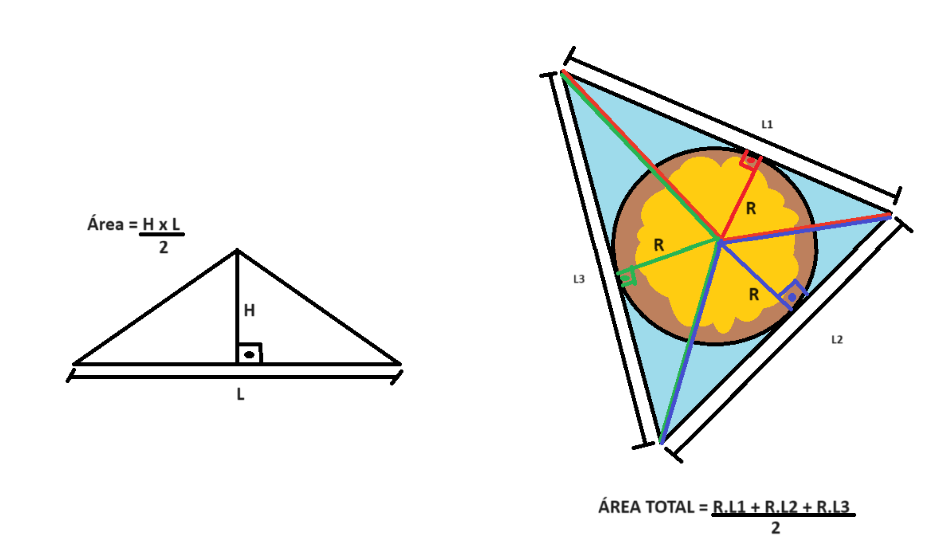
\includegraphics[scale=0.65]{drawkcab/editorial.png}
\end{center}

O próximo passo é determinar o maior valor total possível para cada substring
palindrome maximal. Note que, para substrings de tamanho par, isto é dado por
duas vezes a soma do prefixo de maior soma na segunda metade da substring, e
que, para substrings de tamanho ímpar, é dado por essa soma mais o valor da
letra em seu centro. Na figura exemplificada acima, a resposta é dada por duas vezes a soma do prefixo de maior
soma em $[-10,15,11,-20]$ (que é 16, dado pela soma de $[-10,15,11]$).

Esta soma
pode ser obtida em $O(\lg N)$ através da construção de uma Árvore de
Segmentos adaptada para responder essas consultas, conforme descrito em [2].

Complexidade total: $O(N\lg N)$.

[1] \url{https://cp-algorithms.com/string/manacher.html}

[2] \url{https://www.geeksforgeeks.org/maximum-prefix-sum-given-range/}

\lstinputlisting[title=\large\textbf{double-casting.cpp}, style=cppStyle]{double_casting/double_casting.cpp}

\newpage
\section*{E: Estresse} %tle=1
O algoritmo de Manacher[1] encontra, para cada posição $i$ da string, o maior
valor de $j$ tal que $s[i-j..i+j]$ é palíndrome, e o maior valor de $j'$ tal que
$s[i-j'+1..i+j']$ é palíndrome (isto é, o algoritmo consegue determinar, para cada
posição da string, o tamanho da substring palíndrome maximal cujo centro ocorre
naquela posição, tanto a de tamanho ímpar ($j$) quanto a de tamanho par ($j'$)). O algoritmo tem complexidade $O(N)$.

A figura abaixo exemplifica a solução para o exemplo dado no enunciado. O
tamanho obtido pelo algoritmo de Manacher é representado em vermelho:

\begin{center}
    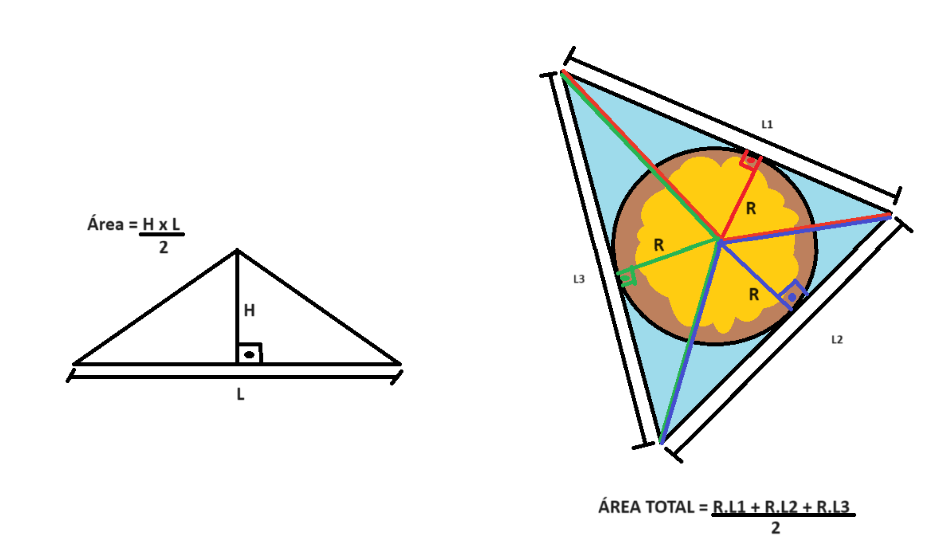
\includegraphics[scale=0.65]{drawkcab/editorial.png}
\end{center}

O próximo passo é determinar o maior valor total possível para cada substring
palindrome maximal. Note que, para substrings de tamanho par, isto é dado por
duas vezes a soma do prefixo de maior soma na segunda metade da substring, e
que, para substrings de tamanho ímpar, é dado por essa soma mais o valor da
letra em seu centro. Na figura exemplificada acima, a resposta é dada por duas vezes a soma do prefixo de maior
soma em $[-10,15,11,-20]$ (que é 16, dado pela soma de $[-10,15,11]$).

Esta soma
pode ser obtida em $O(\lg N)$ através da construção de uma Árvore de
Segmentos adaptada para responder essas consultas, conforme descrito em [2].

Complexidade total: $O(N\lg N)$.

[1] \url{https://cp-algorithms.com/string/manacher.html}

[2] \url{https://www.geeksforgeeks.org/maximum-prefix-sum-given-range/}

\lstinputlisting[title=\large\textbf{estresse.cpp}, style=cppStyle]{estresse/estresse-editorial.cpp}

%\newpage
%\section*{F: Futebol} %tle=1
%O algoritmo de Manacher[1] encontra, para cada posição $i$ da string, o maior
valor de $j$ tal que $s[i-j..i+j]$ é palíndrome, e o maior valor de $j'$ tal que
$s[i-j'+1..i+j']$ é palíndrome (isto é, o algoritmo consegue determinar, para cada
posição da string, o tamanho da substring palíndrome maximal cujo centro ocorre
naquela posição, tanto a de tamanho ímpar ($j$) quanto a de tamanho par ($j'$)). O algoritmo tem complexidade $O(N)$.

A figura abaixo exemplifica a solução para o exemplo dado no enunciado. O
tamanho obtido pelo algoritmo de Manacher é representado em vermelho:

\begin{center}
    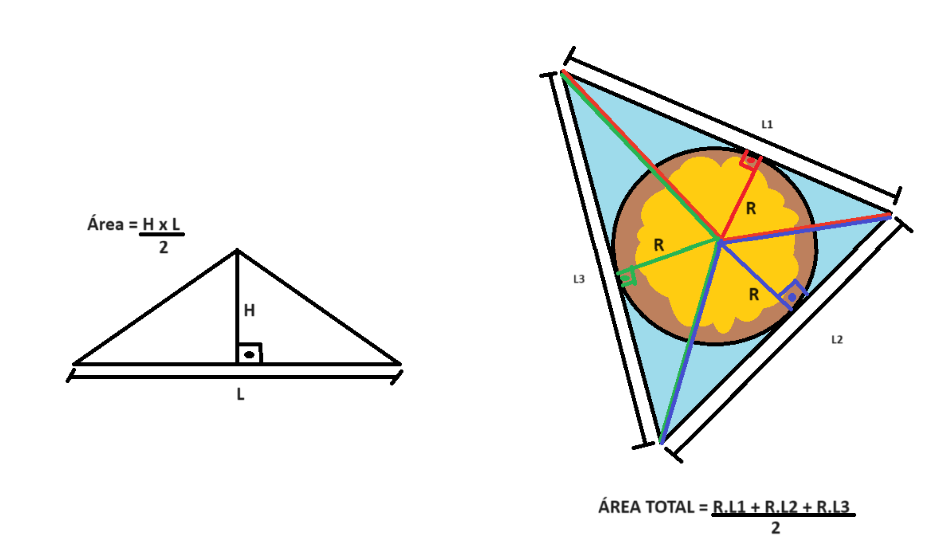
\includegraphics[scale=0.65]{drawkcab/editorial.png}
\end{center}

O próximo passo é determinar o maior valor total possível para cada substring
palindrome maximal. Note que, para substrings de tamanho par, isto é dado por
duas vezes a soma do prefixo de maior soma na segunda metade da substring, e
que, para substrings de tamanho ímpar, é dado por essa soma mais o valor da
letra em seu centro. Na figura exemplificada acima, a resposta é dada por duas vezes a soma do prefixo de maior
soma em $[-10,15,11,-20]$ (que é 16, dado pela soma de $[-10,15,11]$).

Esta soma
pode ser obtida em $O(\lg N)$ através da construção de uma Árvore de
Segmentos adaptada para responder essas consultas, conforme descrito em [2].

Complexidade total: $O(N\lg N)$.

[1] \url{https://cp-algorithms.com/string/manacher.html}

[2] \url{https://www.geeksforgeeks.org/maximum-prefix-sum-given-range/}

%\lstinputlisting[title=\large\textbf{futebol.cpp}, style=cppStyle]{futebol/futebol.cpp}

%\newpage
%\section*{G: Graffiti} %tle=1
%O algoritmo de Manacher[1] encontra, para cada posição $i$ da string, o maior
valor de $j$ tal que $s[i-j..i+j]$ é palíndrome, e o maior valor de $j'$ tal que
$s[i-j'+1..i+j']$ é palíndrome (isto é, o algoritmo consegue determinar, para cada
posição da string, o tamanho da substring palíndrome maximal cujo centro ocorre
naquela posição, tanto a de tamanho ímpar ($j$) quanto a de tamanho par ($j'$)). O algoritmo tem complexidade $O(N)$.

A figura abaixo exemplifica a solução para o exemplo dado no enunciado. O
tamanho obtido pelo algoritmo de Manacher é representado em vermelho:

\begin{center}
    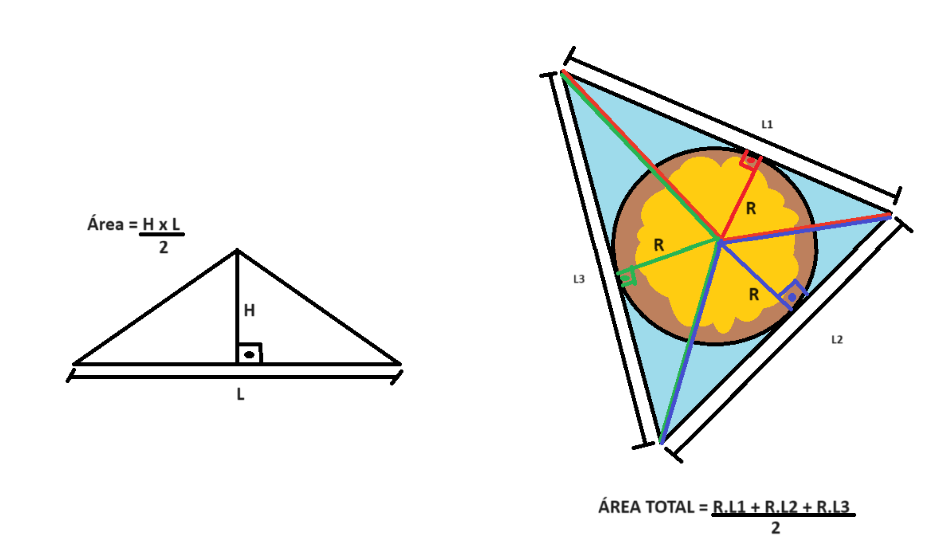
\includegraphics[scale=0.65]{drawkcab/editorial.png}
\end{center}

O próximo passo é determinar o maior valor total possível para cada substring
palindrome maximal. Note que, para substrings de tamanho par, isto é dado por
duas vezes a soma do prefixo de maior soma na segunda metade da substring, e
que, para substrings de tamanho ímpar, é dado por essa soma mais o valor da
letra em seu centro. Na figura exemplificada acima, a resposta é dada por duas vezes a soma do prefixo de maior
soma em $[-10,15,11,-20]$ (que é 16, dado pela soma de $[-10,15,11]$).

Esta soma
pode ser obtida em $O(\lg N)$ através da construção de uma Árvore de
Segmentos adaptada para responder essas consultas, conforme descrito em [2].

Complexidade total: $O(N\lg N)$.

[1] \url{https://cp-algorithms.com/string/manacher.html}

[2] \url{https://www.geeksforgeeks.org/maximum-prefix-sum-given-range/}

%\lstinputlisting[title=\large\textbf{graffiti.cpp}, style=cppStyle]{graffiti/graffiti.cpp}

%\newpage
%\section*{H: Herança} %tle=1
%O algoritmo de Manacher[1] encontra, para cada posição $i$ da string, o maior
valor de $j$ tal que $s[i-j..i+j]$ é palíndrome, e o maior valor de $j'$ tal que
$s[i-j'+1..i+j']$ é palíndrome (isto é, o algoritmo consegue determinar, para cada
posição da string, o tamanho da substring palíndrome maximal cujo centro ocorre
naquela posição, tanto a de tamanho ímpar ($j$) quanto a de tamanho par ($j'$)). O algoritmo tem complexidade $O(N)$.

A figura abaixo exemplifica a solução para o exemplo dado no enunciado. O
tamanho obtido pelo algoritmo de Manacher é representado em vermelho:

\begin{center}
    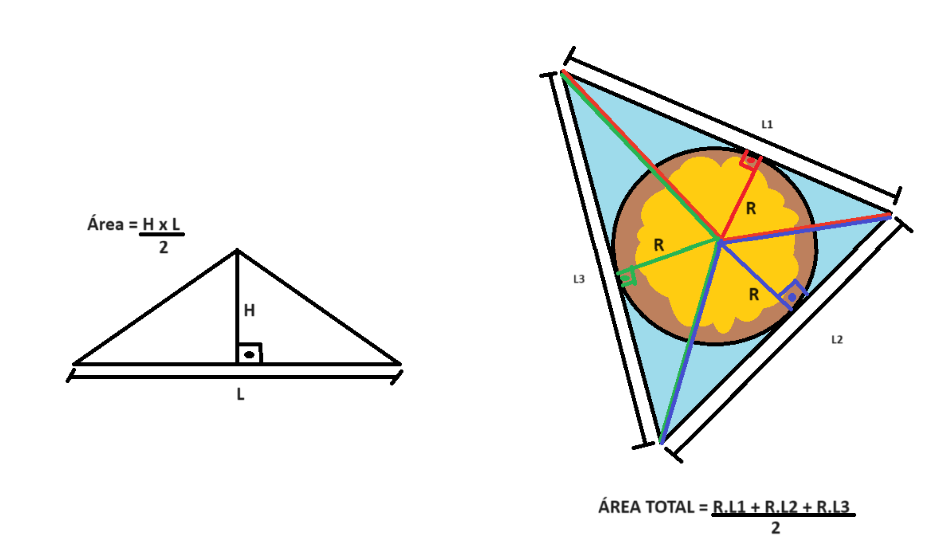
\includegraphics[scale=0.65]{drawkcab/editorial.png}
\end{center}

O próximo passo é determinar o maior valor total possível para cada substring
palindrome maximal. Note que, para substrings de tamanho par, isto é dado por
duas vezes a soma do prefixo de maior soma na segunda metade da substring, e
que, para substrings de tamanho ímpar, é dado por essa soma mais o valor da
letra em seu centro. Na figura exemplificada acima, a resposta é dada por duas vezes a soma do prefixo de maior
soma em $[-10,15,11,-20]$ (que é 16, dado pela soma de $[-10,15,11]$).

Esta soma
pode ser obtida em $O(\lg N)$ através da construção de uma Árvore de
Segmentos adaptada para responder essas consultas, conforme descrito em [2].

Complexidade total: $O(N\lg N)$.

[1] \url{https://cp-algorithms.com/string/manacher.html}

[2] \url{https://www.geeksforgeeks.org/maximum-prefix-sum-given-range/}

%\lstinputlisting[title=\large\textbf{heranca.cpp}, style=cppStyle]{heranca/heranca.cpp}

\newpage
\section*{I: Ímpar e Impares} %tle=1
O algoritmo de Manacher[1] encontra, para cada posição $i$ da string, o maior
valor de $j$ tal que $s[i-j..i+j]$ é palíndrome, e o maior valor de $j'$ tal que
$s[i-j'+1..i+j']$ é palíndrome (isto é, o algoritmo consegue determinar, para cada
posição da string, o tamanho da substring palíndrome maximal cujo centro ocorre
naquela posição, tanto a de tamanho ímpar ($j$) quanto a de tamanho par ($j'$)). O algoritmo tem complexidade $O(N)$.

A figura abaixo exemplifica a solução para o exemplo dado no enunciado. O
tamanho obtido pelo algoritmo de Manacher é representado em vermelho:

\begin{center}
    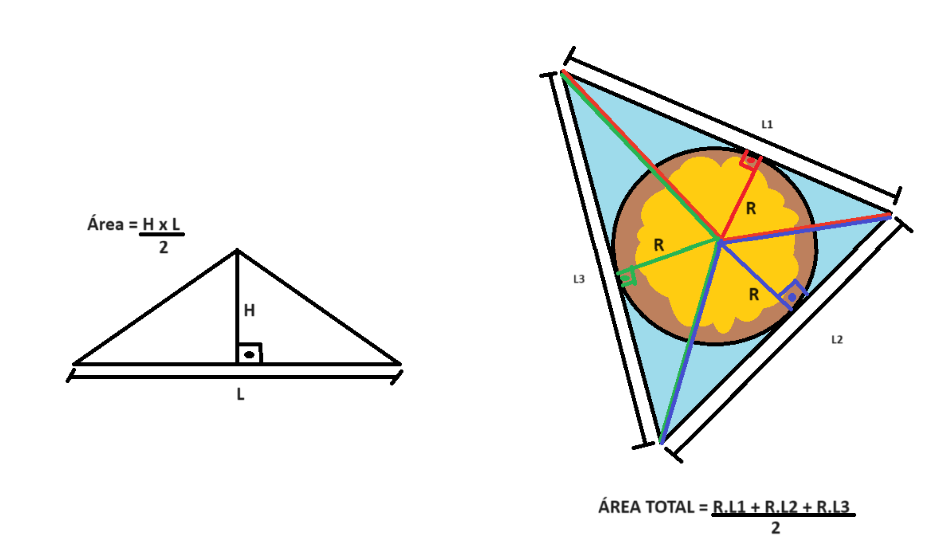
\includegraphics[scale=0.65]{drawkcab/editorial.png}
\end{center}

O próximo passo é determinar o maior valor total possível para cada substring
palindrome maximal. Note que, para substrings de tamanho par, isto é dado por
duas vezes a soma do prefixo de maior soma na segunda metade da substring, e
que, para substrings de tamanho ímpar, é dado por essa soma mais o valor da
letra em seu centro. Na figura exemplificada acima, a resposta é dada por duas vezes a soma do prefixo de maior
soma em $[-10,15,11,-20]$ (que é 16, dado pela soma de $[-10,15,11]$).

Esta soma
pode ser obtida em $O(\lg N)$ através da construção de uma Árvore de
Segmentos adaptada para responder essas consultas, conforme descrito em [2].

Complexidade total: $O(N\lg N)$.

[1] \url{https://cp-algorithms.com/string/manacher.html}

[2] \url{https://www.geeksforgeeks.org/maximum-prefix-sum-given-range/}

\lstinputlisting[title=\large\textbf{impar-e-impares.cpp}, style=cppStyle]{impar_e_impares/impar_e_impares.cpp}

%\newpage
%\section*{J: Joias do Tesouro} %tle=1
%O algoritmo de Manacher[1] encontra, para cada posição $i$ da string, o maior
valor de $j$ tal que $s[i-j..i+j]$ é palíndrome, e o maior valor de $j'$ tal que
$s[i-j'+1..i+j']$ é palíndrome (isto é, o algoritmo consegue determinar, para cada
posição da string, o tamanho da substring palíndrome maximal cujo centro ocorre
naquela posição, tanto a de tamanho ímpar ($j$) quanto a de tamanho par ($j'$)). O algoritmo tem complexidade $O(N)$.

A figura abaixo exemplifica a solução para o exemplo dado no enunciado. O
tamanho obtido pelo algoritmo de Manacher é representado em vermelho:

\begin{center}
    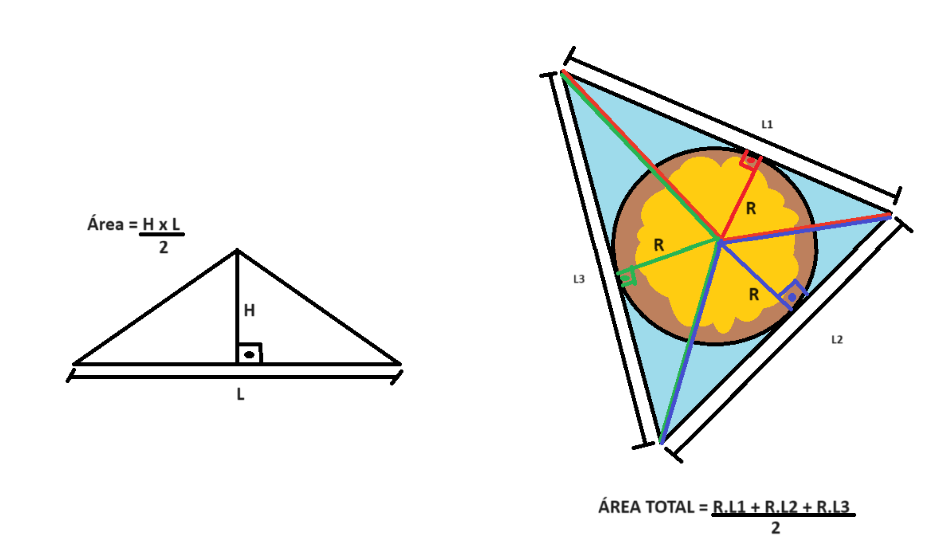
\includegraphics[scale=0.65]{drawkcab/editorial.png}
\end{center}

O próximo passo é determinar o maior valor total possível para cada substring
palindrome maximal. Note que, para substrings de tamanho par, isto é dado por
duas vezes a soma do prefixo de maior soma na segunda metade da substring, e
que, para substrings de tamanho ímpar, é dado por essa soma mais o valor da
letra em seu centro. Na figura exemplificada acima, a resposta é dada por duas vezes a soma do prefixo de maior
soma em $[-10,15,11,-20]$ (que é 16, dado pela soma de $[-10,15,11]$).

Esta soma
pode ser obtida em $O(\lg N)$ através da construção de uma Árvore de
Segmentos adaptada para responder essas consultas, conforme descrito em [2].

Complexidade total: $O(N\lg N)$.

[1] \url{https://cp-algorithms.com/string/manacher.html}

[2] \url{https://www.geeksforgeeks.org/maximum-prefix-sum-given-range/}

%\lstinputlisting[title=\large\textbf{joias.cpp}, style=cppStyle]{joias/joias.cpp}

\newpage
\section*{K: Kleber e a Convenção} %tle=1
O algoritmo de Manacher[1] encontra, para cada posição $i$ da string, o maior
valor de $j$ tal que $s[i-j..i+j]$ é palíndrome, e o maior valor de $j'$ tal que
$s[i-j'+1..i+j']$ é palíndrome (isto é, o algoritmo consegue determinar, para cada
posição da string, o tamanho da substring palíndrome maximal cujo centro ocorre
naquela posição, tanto a de tamanho ímpar ($j$) quanto a de tamanho par ($j'$)). O algoritmo tem complexidade $O(N)$.

A figura abaixo exemplifica a solução para o exemplo dado no enunciado. O
tamanho obtido pelo algoritmo de Manacher é representado em vermelho:

\begin{center}
    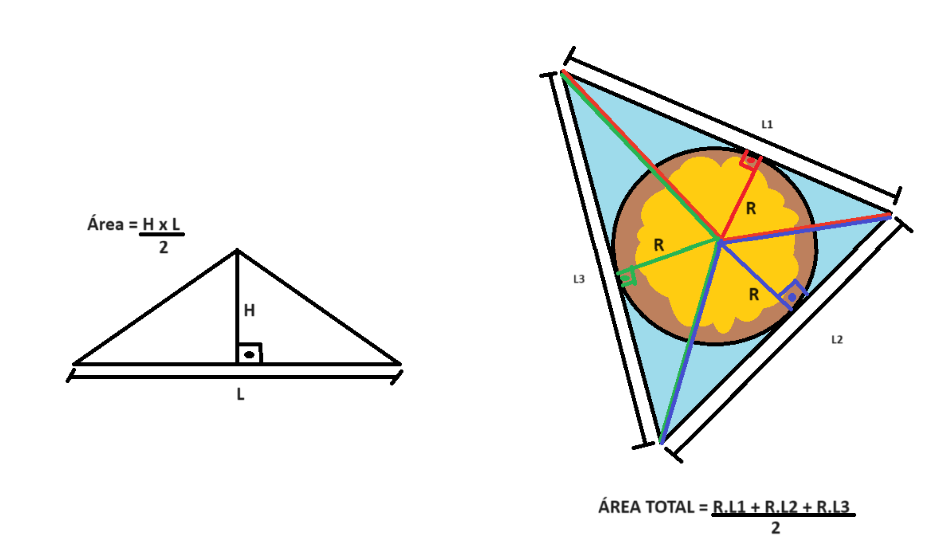
\includegraphics[scale=0.65]{drawkcab/editorial.png}
\end{center}

O próximo passo é determinar o maior valor total possível para cada substring
palindrome maximal. Note que, para substrings de tamanho par, isto é dado por
duas vezes a soma do prefixo de maior soma na segunda metade da substring, e
que, para substrings de tamanho ímpar, é dado por essa soma mais o valor da
letra em seu centro. Na figura exemplificada acima, a resposta é dada por duas vezes a soma do prefixo de maior
soma em $[-10,15,11,-20]$ (que é 16, dado pela soma de $[-10,15,11]$).

Esta soma
pode ser obtida em $O(\lg N)$ através da construção de uma Árvore de
Segmentos adaptada para responder essas consultas, conforme descrito em [2].

Complexidade total: $O(N\lg N)$.

[1] \url{https://cp-algorithms.com/string/manacher.html}

[2] \url{https://www.geeksforgeeks.org/maximum-prefix-sum-given-range/}

\lstinputlisting[title=\large\textbf{kleber-e-a-convencao.cpp}, style=cppStyle]{kleber_e_a_convencao/ac.cpp}

%\newpage
%\section*{L: Lâmpada Maldita} %tle=1
%O algoritmo de Manacher[1] encontra, para cada posição $i$ da string, o maior
valor de $j$ tal que $s[i-j..i+j]$ é palíndrome, e o maior valor de $j'$ tal que
$s[i-j'+1..i+j']$ é palíndrome (isto é, o algoritmo consegue determinar, para cada
posição da string, o tamanho da substring palíndrome maximal cujo centro ocorre
naquela posição, tanto a de tamanho ímpar ($j$) quanto a de tamanho par ($j'$)). O algoritmo tem complexidade $O(N)$.

A figura abaixo exemplifica a solução para o exemplo dado no enunciado. O
tamanho obtido pelo algoritmo de Manacher é representado em vermelho:

\begin{center}
    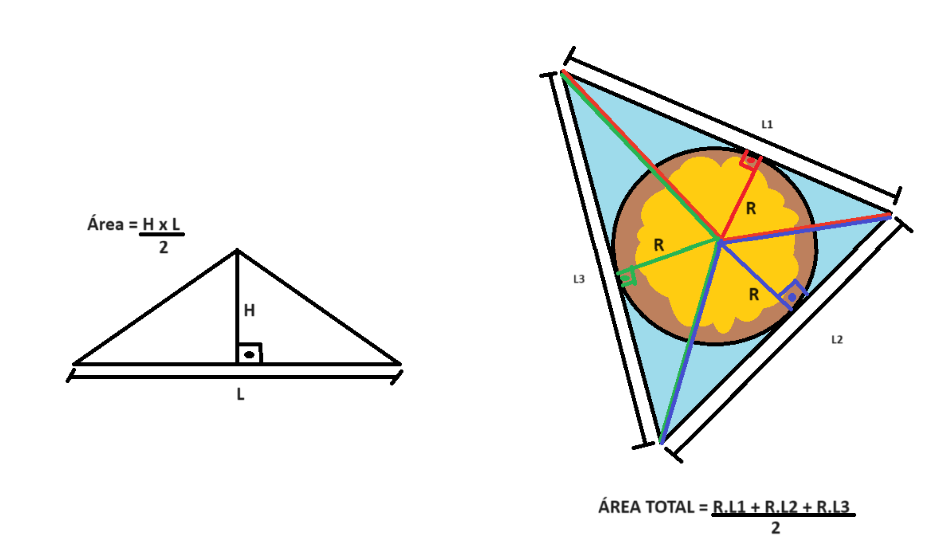
\includegraphics[scale=0.65]{drawkcab/editorial.png}
\end{center}

O próximo passo é determinar o maior valor total possível para cada substring
palindrome maximal. Note que, para substrings de tamanho par, isto é dado por
duas vezes a soma do prefixo de maior soma na segunda metade da substring, e
que, para substrings de tamanho ímpar, é dado por essa soma mais o valor da
letra em seu centro. Na figura exemplificada acima, a resposta é dada por duas vezes a soma do prefixo de maior
soma em $[-10,15,11,-20]$ (que é 16, dado pela soma de $[-10,15,11]$).

Esta soma
pode ser obtida em $O(\lg N)$ através da construção de uma Árvore de
Segmentos adaptada para responder essas consultas, conforme descrito em [2].

Complexidade total: $O(N\lg N)$.

[1] \url{https://cp-algorithms.com/string/manacher.html}

[2] \url{https://www.geeksforgeeks.org/maximum-prefix-sum-given-range/}

%\lstinputlisting[title=\large\textbf{lampada.cpp}, style=cppStyle]{lampada/lampada.cpp}

\end{document}
